\documentclass[10pt, a4paper]{article}

% ── Packages ──────────────────────────────────────────────────────────────────
\usepackage[a4paper, top=2.5cm, bottom=2.5cm, left=1.8cm, right=1.8cm]{geometry}
\usepackage{xcolor}
\usepackage{titlesec}
\usepackage{graphicx}
\usepackage{booktabs}
\usepackage{array}
\usepackage{multirow}
\usepackage{amsmath}
\usepackage{amssymb}
\usepackage{hyperref}
\usepackage{enumitem}
\usepackage{microtype}
\usepackage{fancyhdr}
\usepackage{tcolorbox}
\usepackage{listings}
\usepackage{caption}
\usepackage{float}
\usepackage{times}
\usepackage{parskip}
\usepackage{tabularx}

\tcbuselibrary{skins, breakable}

% ── Colors ────────────────────────────────────────────────────────────────────
\definecolor{navyblue}{RGB}{26, 50, 89}
\definecolor{lightgray}{RGB}{245, 245, 245}
\definecolor{linkblue}{RGB}{0, 102, 204}

% ── Section Styling (full-width colored box, white text) ──────────────────────


\titleformat{\subsection}
  {\normalfont\normalsize\bfseries}
  {\thesubsection}
  {0.5em}
  {}
\titlespacing*{\subsection}{0pt}{8pt}{3pt}

% ── Hyperlinks ────────────────────────────────────────────────────────────────
\hypersetup{colorlinks=true, linkcolor=linkblue, urlcolor=linkblue, citecolor=linkblue}

% ── Header / Footer ───────────────────────────────────────────────────────────
\pagestyle{fancy}
\fancyhf{}
\rhead{\small EE200}
\lhead{\small Question 3 Report}
\cfoot{\small \thepage}
\renewcommand{\headrulewidth}{0.4pt}

% ── Table & Caption ───────────────────────────────────────────────────────────
\renewcommand{\arraystretch}{1.3}
\captionsetup{font=small, labelfont=bf, skip=4pt}

% ── Code listing ──────────────────────────────────────────────────────────────
\lstset{
  backgroundcolor=\color{lightgray},
  basicstyle=\ttfamily\scriptsize,
  breaklines=true,
  frame=single,
  numbers=left,
  numberstyle=\tiny\color{gray},
  keywordstyle=\color{navyblue}\bfseries,
  commentstyle=\color{gray}\itshape,
}

% ── Closed-border table helper ────────────────────────────────────────────────
% Use \hline at top, \hline between rows, \hline at bottom, with | for vertical lines

% ─────────────────────────────────────────────────────────────────────────────
\begin{document}

  \begin{center}
    \vspace{2.0cm}
    {\LARGE \textbf{EE200: Signals, Systems and Networks}}\\[4pt]
    {\LARGE \textbf{Course Project}}\\[10pt]
    {\Large \textsc{Question 3 Report}}\\[40pt]







    \Large\textsc{Team Members:}\\[10pt]

    \makebox[0.3\textwidth][l]{\textbf{240622 Manish Kajla}}\\
    \makebox[0.3\textwidth][l]{\textbf{241114 Utkarsh Aman}}\\[90pt]

    

    \Large{\textbf{Abstract}}\\[15pt]
    \begin{minipage}{0.90\textwidth}
      \large\itshape\centering
      

        This project explores the development of a Shazam-inspired audio recognition system based on spectrogram analysis and audio fingerprinting. The objective is to identify songs from short and potentially noisy audio clips by extracting distinctive frequency-time characteristics rather than comparing raw audio signals directly. The process begins with transforming audio recordings into spectrograms using the Short-Time Fourier Transform (STFT), providing a time-varying representation of frequency content. Prominent spectral peaks are then detected and represented as constellation maps, capturing the most significant acoustic features of a song. These peaks are paired to generate compact fingerprints that remain robust under noise and minor distortions. A database of fingerprints is constructed for a collection of songs, and unknown audio clips are identified by matching their fingerprints against the stored database and analyzing offset consistency. The project further investigates the impact of noise, time shifts, and spectrogram parameter choices on recognition performance, highlighting the trade-off between time and frequency resolution. Finally, the fingerprinting pipeline is integrated into a simple software application capable of indexing songs and recognizing query clips. The results demonstrate how sparse spectral features can provide accurate, efficient, and noise-resistant audio identification, illustrating the core principles behind modern music recognition systems.
        

    \end{minipage}\\[12pt]
   
    \vspace{0.2cm}
  \end{center}

\vspace{0.5cm}

\noindent\textbf{Live Streamlit App:} \\
\url{https://audio-fingerprinting-241114-240622.streamlit.app/}

\vspace{0.2cm}

\noindent\textbf{Alternate Streamlit App (if the above link is unavailable):} \\
\url{https://audio-fingerprinting-240622-241114.streamlit.app/}

\vspace{0.2cm}

\noindent\textbf{Source Code Repository:} \\
\url{https://github.com/Utkarsh-Aman/Audio-Fingerprinting}
\newpage



\tableofcontents

\newpage

\section{1. The Limitation of a Single Fourier Transform}
To understand why a single Fourier transform is insufficient for audio fingerprinting, we computed the Discrete Fourier Transform (DFT) magnitude of an entire song ("Yesterday"). As shown in Figure \ref{fig:dft}, the DFT provides a global frequency profile, revealing which frequencies are present overall. However, all sense of timing is completely lost. A note played at the beginning of the song and a note played at the end are indistinguishable in this global spectrum. For fingerprinting, we need to know \textit{when} specific frequencies occur.

\begin{figure}[H]
    \centering
    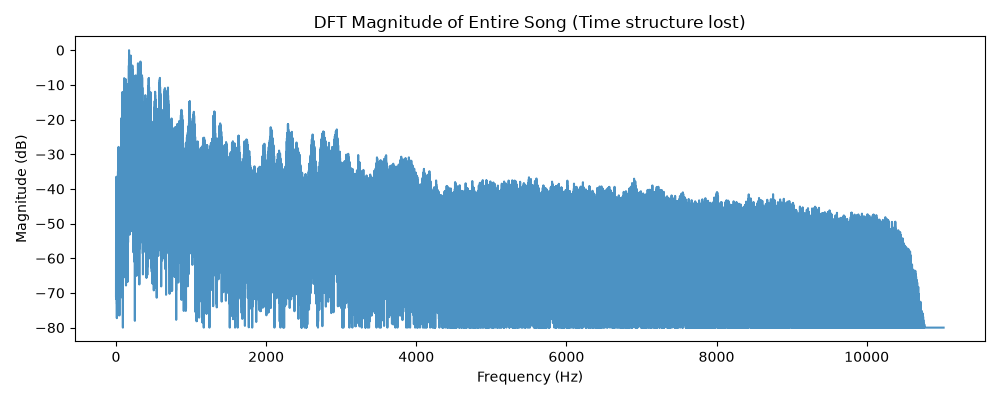
\includegraphics[width=\textwidth]{plots/dft_entire_song.png}
    \caption{DFT Magnitude of an entire song. The time axis is collapsed.}
    \label{fig:dft}
\end{figure}

\section{2. The Spectrogram and Time-Frequency Resolution}
To capture both time and frequency information, we use a spectrogram. By sliding a short window across the signal, computing the DFT for each slice, and stacking the results, we can watch frequency content evolve over time.

We compared spectrograms computed with a short window ($N\_FFT=512$) and a long window ($N\_FFT=8192$), shown in Figure \ref{fig:spectrograms}. This demonstrates the fundamental time-frequency tradeoff (the uncertainty principle):
\begin{itemize}
    \item \textbf{Short Window}: Provides excellent time resolution, allowing us to pinpoint fast transient events (like drum hits) sharply in time. However, frequency bins are wide, resulting in poor frequency resolution (horizontal smearing).
    \item \textbf{Long Window}: Provides excellent frequency resolution, separating closely spaced pitches clearly. However, time resolution degrades, smearing transient events across a wide time region.
\end{itemize}
For fingerprinting, we settle on a middle ground (e.g., $N\_FFT=4096$) that balances localizing peaks in time while resolving musical pitches.

\begin{figure}[H]
    \centering
    \begin{subfigure}{\textwidth}
        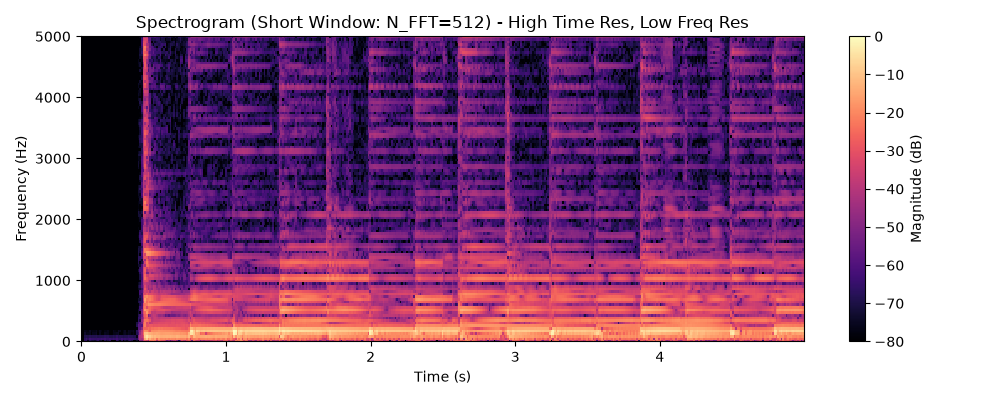
\includegraphics[width=\textwidth]{plots/spectrogram_short.png}
    \end{subfigure}
    \vspace{0.5cm}
    \begin{subfigure}{\textwidth}
        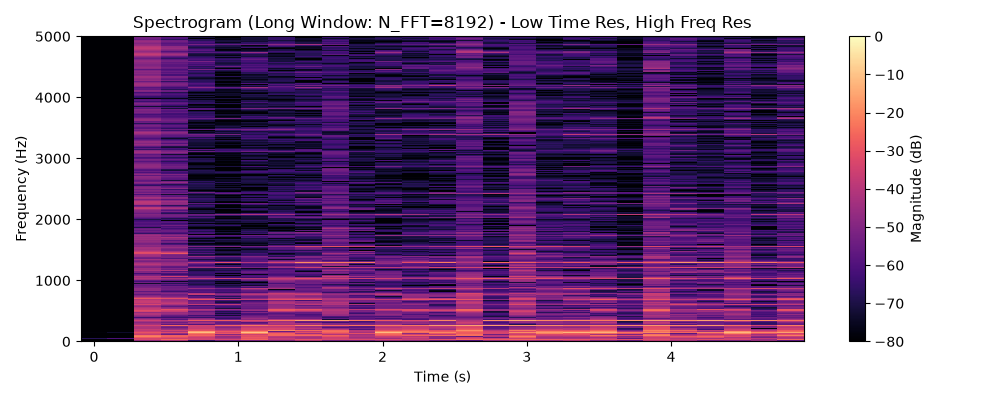
\includegraphics[width=\textwidth]{plots/spectrogram_long.png}
    \end{subfigure}
    \caption{Comparison of short window (top) and long window (bottom) spectrograms, illustrating the time-frequency tradeoff.}
    \label{fig:spectrograms}
\end{figure}

\section{3. Constellation Map (Peak Picking)}
The fingerprint relies on a sparse set of standout points rather than the entire dense spectrogram. We extract local maxima (peaks) from the spectrogram magnitude. A peak is defined as a point that is louder than its immediate neighbors in a small 2D time-frequency window, and above a minimum amplitude threshold (to ignore background noise).

Figure \ref{fig:constellation} shows the extracted constellation map overlaid on the spectrogram. Extracting local maxima ensures peaks are spread across the entire clip's structural features, rather than clumping around a single globally loud event.

\begin{figure}[H]
    \centering
    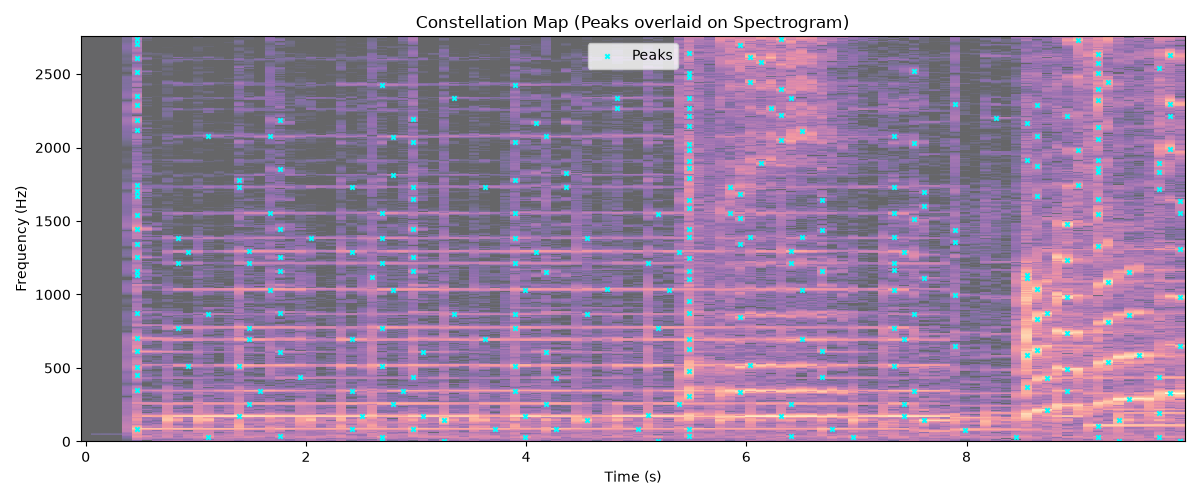
\includegraphics[width=\textwidth]{plots/constellation_map.png}
    \caption{Constellation map: local maxima (cyan crosses) overlaid on the spectrogram.}
    \label{fig:constellation}
\end{figure}

\section{4. Hash Generation and Pairing}
A single peak $(time, frequency)$ is not highly unique across a large database of songs. To create a robust signature, we pair nearby peaks into compact hashes: $(f_{anchor}, f_{target}, \Delta t)$, where $\Delta t$ is the time gap between the anchor peak and target peak. This combinatorial pairing creates highly specific fingerprints that dramatically reduce false collisions.

\section{5. Identification and Offset Matching}
To identify a query clip, we fingerprint it to extract hashes and look up those hashes in our database. For every matching hash, we compute the relative time offset between the database occurrence and the query occurrence: $Offset = t_{database} - t_{query}$. 

Figure \ref{fig:offset_paired} shows the offset histograms for a correct match versus an incorrect candidate. Because the query is a time-shifted excerpt of the true song, all correct hash matches vote for the \textit{same} time offset, creating a massive, sharp spike. Conversely, random hash collisions with an incorrect song scatter randomly across many offsets.

\begin{figure}[H]
    \centering
    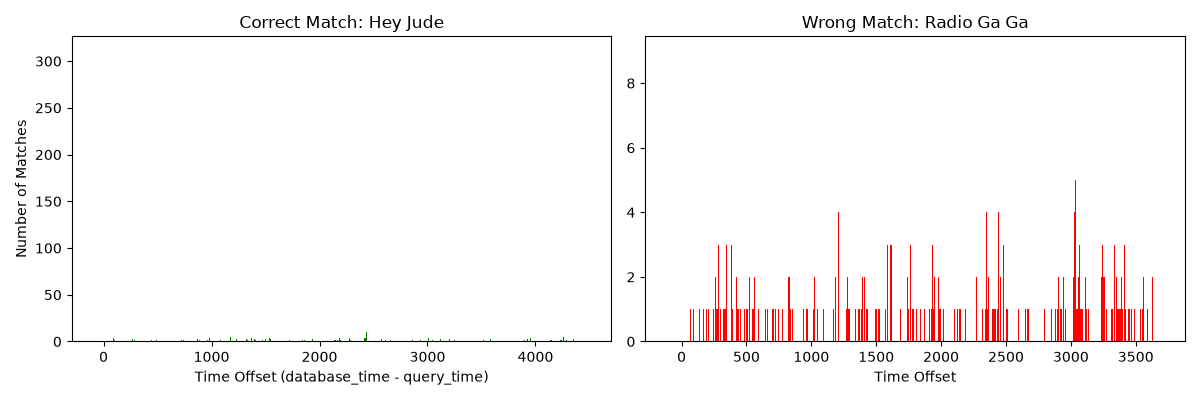
\includegraphics[width=\textwidth]{plots/offset_histogram_paired.png}
    \caption{Offset histograms for paired hashes. The correct match (left) shows a decisive spike at a consistent offset. The wrong match (right) shows scattered, random noise.}
    \label{fig:offset_paired}
\end{figure}

\section{6. Paired Hashes vs. Single Peaks}
We repeated the identification process using only single-peak matching (e.g., matching just the frequency bin). As shown in Figure \ref{fig:offset_single}, single peaks yield a much flatter histogram with high background noise. The combinatorics of pairing peaks ($f_1, f_2, \Delta t$) forces matches to possess rigid structural relationships, making the correct song's spike vastly more decisive compared to background collision noise.

\begin{figure}[H]
    \centering
    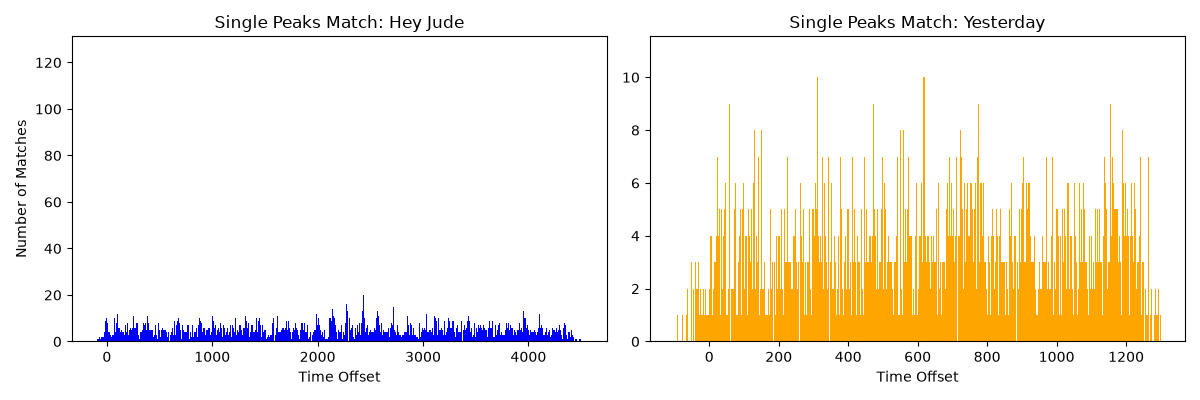
\includegraphics[width=\textwidth]{plots/offset_histogram_single.png}
    \caption{Offset histograms using single-peak matching. The spike is less decisive and the noise floor is much higher.}
    \label{fig:offset_single}
\end{figure}

\section{7. Robustness Testing}

\subsection{a. Noise Robustness}
We added white Gaussian noise at decreasing Signal-to-Noise Ratios (SNR) to a query clip. Figure \ref{fig:robustness_noise} shows that the system remains highly confident even under moderate noise, failing only when the noise entirely buries the dominant structural peaks (e.g., below 0 dB SNR).

\begin{figure}[H]
    \centering
    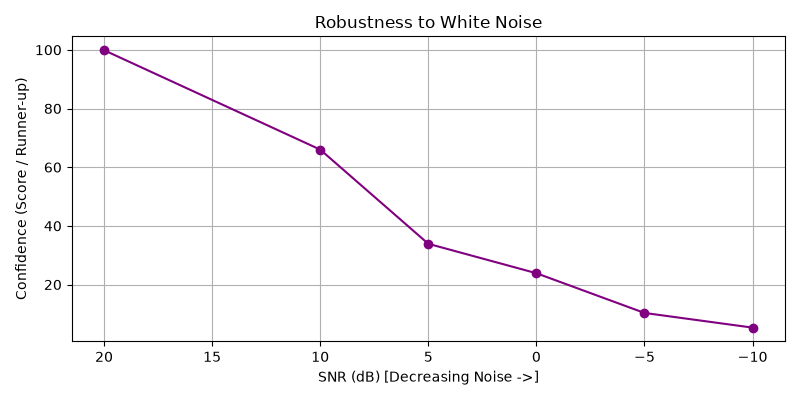
\includegraphics[width=0.8\textwidth]{plots/robustness_noise.png}
    \caption{Identification confidence as a function of SNR.}
    \label{fig:robustness_noise}
\end{figure}

\subsection{b. Pitch Shift Robustness}
We artificially shifted the pitch of the query clip by fractions of a semitone. As Figure \ref{fig:robustness_pitch} shows, even a tiny shift ($\geq 0.5$ semitones) breaks the identifier completely. Although the song sounds perceptually identical to humans, our database hashes rely on \textit{exact} absolute frequency bins. Shifting the pitch moves all peaks vertically out of their recorded bins, causing total hash lookup failure.

\begin{figure}[H]
    \centering
    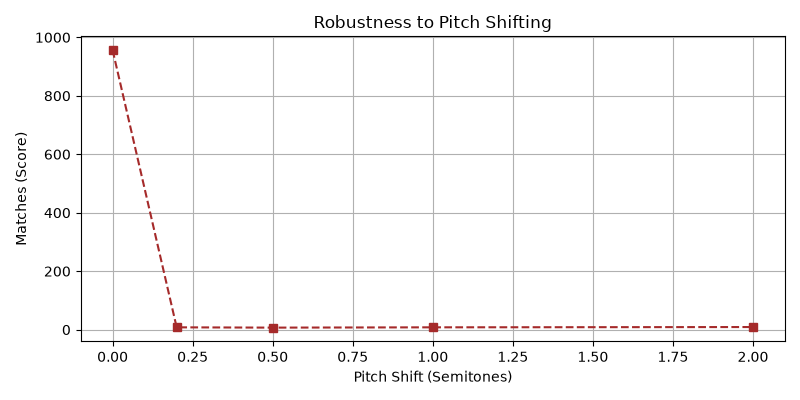
\includegraphics[width=0.8\textwidth]{plots/robustness_pitch.png}
    \caption{Identification score as a function of artificial pitch shifting.}
    \label{fig:robustness_pitch}
\end{figure}

\subsection{c. Proposed Improvements}
To make the system robust to slight pitch variations, one concrete change would be to use \textbf{frequency ratios} ($f_{target} / f_{anchor}$) or logarithmic frequency gaps instead of absolute frequencies in the hash tuple. Because pitch shifting moves all frequencies by a constant multiplicative factor, their ratios remain invariant, allowing hashes to match despite pitch distortions. Alternatively, we could perform \textbf{fuzzy matching} by quantizing frequency bins with a larger tolerance.

\end{document}
